\documentclass[11pt,letterpaper]{article}
\usepackage{fullpage}
\usepackage[top=0.5in, bottom=1.5in, left=1in, right=1in]{geometry}
\usepackage{amsmath,amsthm,amsfonts,amssymb,amscd}
\usepackage{lastpage}
\usepackage{enumerate}
\usepackage{enumitem}
\usepackage{fancyhdr}
\usepackage{graphicx}
\usepackage{listings}
\usepackage{hyperref}
\usepackage{booktabs}
\usepackage{cancel}
\usepackage{physics}
\usepackage{caption,cleveref,colortbl,csquotes,datatool,helvet,mathpazo,multirow,listings,pgfplots,xcolor}

\hypersetup{%
  colorlinks=true,
  linkcolor=blue,
  linkbordercolor={0 0 1}
}

\setlength{\parindent}{0.0in}
\setlength{\parskip}{0.05in}
\setlength{\footnotesep}{1.2\baselineskip}


% edit these
\newcommand\course{AST222H}
\newcommand\Title{Problem Set 2}
\newcommand\Name{Jeff Shen} 
\newcommand\Id{1004911526} 
\newcommand\Date{7 Feb 2020}

\pagestyle{fancyplain}
\headheight 35pt
\lhead{\Name}
\lhead{\Name\\\Id}
\chead{\LARGE \Title}
\rhead{\course \\ \Date}
\lfoot{}
\cfoot{}
\rfoot{\small\thepage}
\pgfplotsset{compat=1.16}
\headsep 1.2em

\begin{document}

% problem 3
\section*{Problem 3}

\subsection*{Galaxy 1}
\begin{figure*}[!htbp]
    \centering
    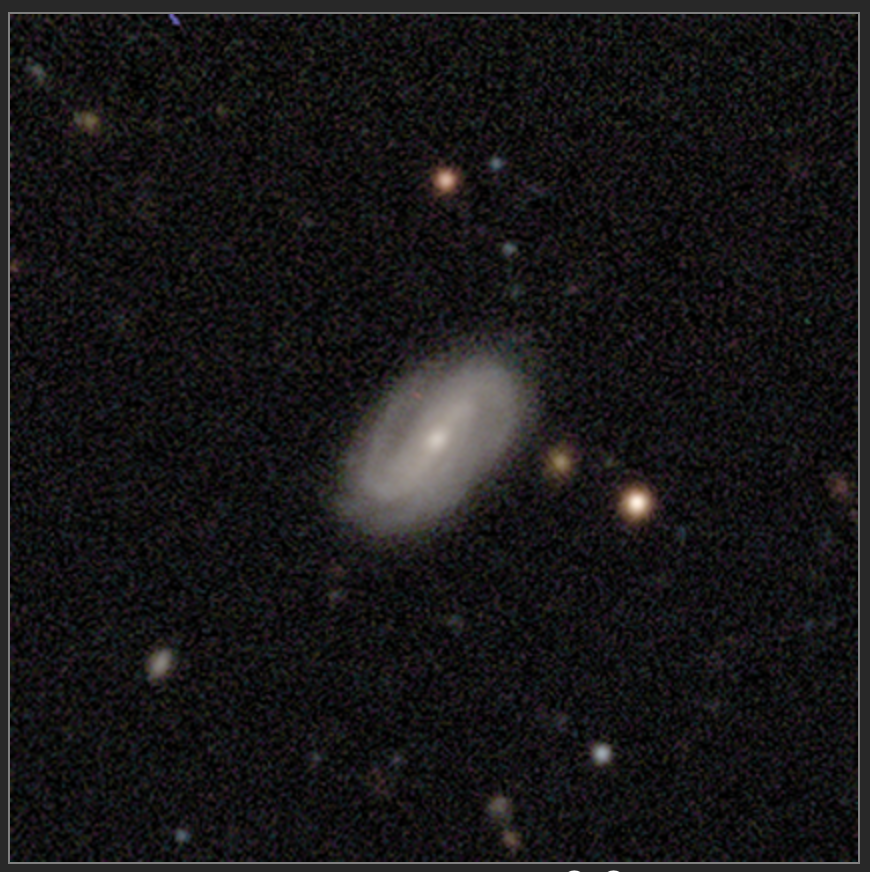
\includegraphics[width=\linewidth]{gal1.png}
\end{figure*}

\newpage

\begin{enumerate}

    \item Is the galaxy simply smooth and rounded, with no sign of a disk?

        Smooth / \fbox{Features or Disk} / Star or Artifact

    \item Could this be a disk viewed edge-on?

Yes - Edge On Disk / \fbox{No - Something Else}

\item Is there a bar feature through the centre of the galaxy?

No Bar / \fbox{Weak Bar} / Strong Bar

\item Is there any sign of a spiral arm pattern?

\fbox{Yes} / No

\item How tightly wound do the spiral arms appear?

Tight / \fbox{Medium} / Loose 

\item How many spiral arms are there?

1 / \fbox{2} / 3 / 4 / More than 4 / Can't tell

\item Is there a central bulge? If so, how large is it compared with the galaxy?

No Bulge / \fbox{Small} / Moderate / Large / Dominant

\item Is the galaxy merging or disturbed?

Merging / Major Disturbance / Minor Disturbance / \fbox{None}

\item Do you see any of these rare features?

    Ring / Lens or arc / Irregular / Dust lane / Overlapping / Something Else / \fbox{Nothing Unusual} 
\end{enumerate}

Hubble type estimation: SBb

\newpage
\subsection*{Galaxy 2}
\begin{figure*}[!htbp]
    \centering
    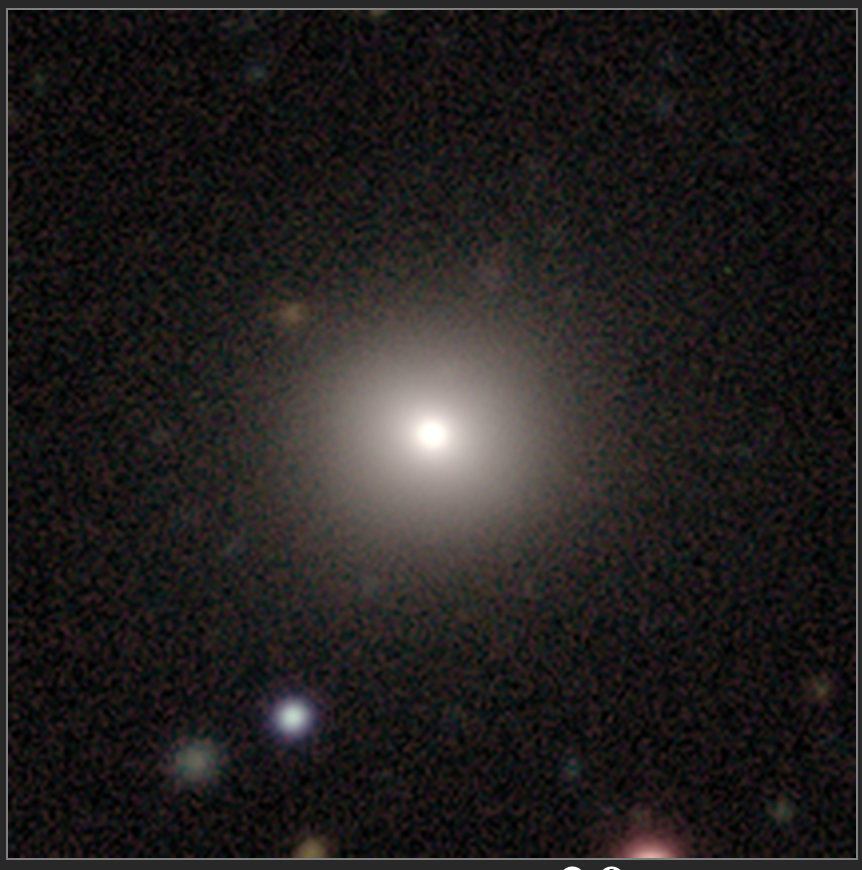
\includegraphics[width=\linewidth]{gal2.png}
\end{figure*}

\newpage

\begin{enumerate}
\item Is the galaxy simply smooth and rounded, with no sign of a disk?

        Smooth / \fbox{Features or Disk} / Star or Artifact

    \item Could this be a disk viewed edge-on?

Yes - Edge On Disk / \fbox{No - Something Else}

\item Is there a bar feature through the centre of the galaxy?

    \fbox{No Bar} / Weak Bar / Strong Bar

\item Is there any sign of a spiral arm pattern?

    Yes / \fbox{No}

\item Is there a central bulge? If so, how large is it compared with the galaxy?

    No Bulge / Small / \fbox{Moderate} / Large / Dominant

\item Is the galaxy merging or disturbed?

Merging / Major Disturbance / Minor Disturbance / \fbox{None}

\item Do you see any of these rare features?

    Ring / Lens or arc / Irregular / Dust lane / Overlapping / Something Else / \fbox{Nothing Unusual} 

\end{enumerate}

Hubble type estimation: E0 

\newpage

\subsection*{Galaxy 3}
\begin{figure*}[!htbp]
    \centering
    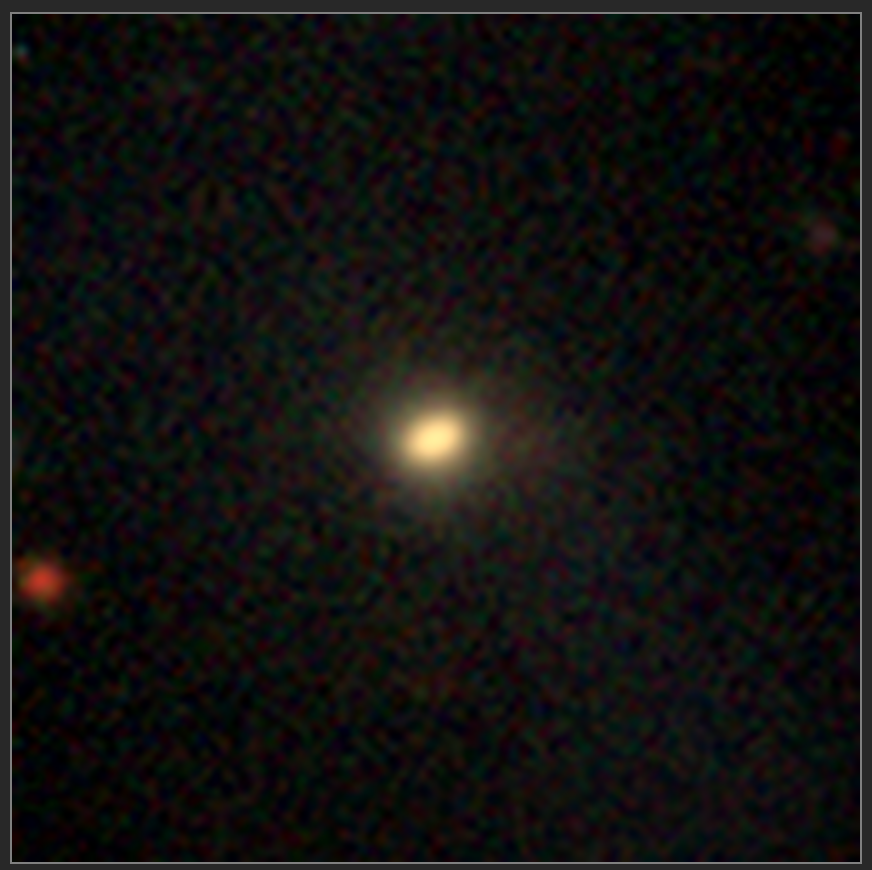
\includegraphics[width=\linewidth]{gal3.png}
\end{figure*}

\newpage

\begin{enumerate}
\item Is the galaxy simply smooth and rounded, with no sign of a disk?

        Smooth / \fbox{Features or Disk} / Star or Artifact

    \item Could this be a disk viewed edge-on?

Yes - Edge On Disk / \fbox{No - Something Else}

\item Is there a bar feature through the centre of the galaxy?

    \fbox{No Bar} / Weak Bar / Strong Bar

\item Is there any sign of a spiral arm pattern?

    Yes / \fbox{No}

\item Is there a central bulge? If so, how large is it compared with the galaxy?

    No Bulge / Small / Moderate / Large / \fbox{Dominant}

\item Is the galaxy merging or disturbed?

Merging / Major Disturbance / Minor Disturbance / \fbox{None}

\item Do you see any of these rare features?

    Ring / Lens or arc / Irregular / Dust lane / Overlapping / Something Else / \fbox{Nothing Unusual} 

\end{enumerate}

Hubble type estimation: S0 
\end{document}
